
%% \begin{figure*}
%%   \centering
%%   \subfloat[Optimizer Sensitivity]{
%%     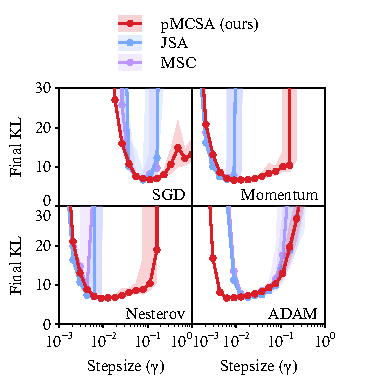
\includegraphics[scale=1.0]{figures/stepsize_01.pdf}
%%   } \\
%%   \subfloat[Gradient Variance]{
%%     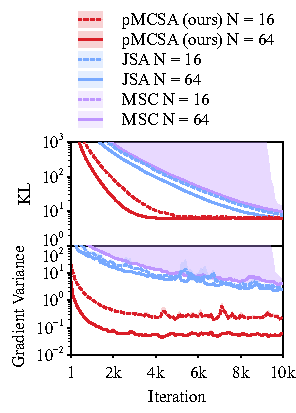
\includegraphics[scale=1.0]{figures/gaussian_01.pdf}
%%   }
%%   \caption{\textbf{Optimizer stepsize (\(\gamma\)) versus final KL. pMCSA is the least sensitive to optimizer hyperparameters and results in stable convergence.}
%%       The final KL is obtained at the \(10^4\)th iteration.
%%       The target distribution is a 100-D Gaussian with \(\nu = 500\).
%%       The error bands are the 80\% quantiles while the solid lines are the median of 20 replications.
%%   }
%% \end{figure*}

\begin{figure*}
  \vspace{-0.2in}
  \centering
  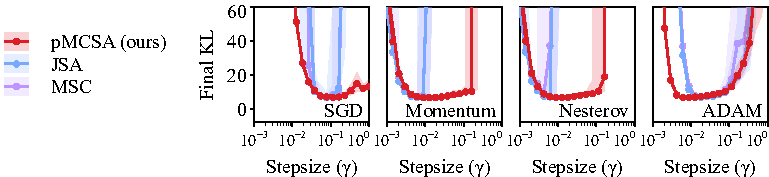
\includegraphics[scale=0.9]{figures/stepsize_02.pdf}
  \vspace{-0.05in}
  \caption{\textbf{Optimizer stepsize (\(\gamma\)) versus final KL.
      pMCSA is the least sensitive to optimizer hyperparameters and results in stable convergence.}
      The final KL is obtained at the \(10^4\)th iteration.
      The target distribution is a 100-D Gaussian with \(\nu = 500\).
      The error bands are the 80\% quantiles while the solid lines are the median of 20 replications.
  }\label{fig:stepsize}
\end{figure*}
\begin{figure*}
  \vspace{-0.1in}
  \centering
  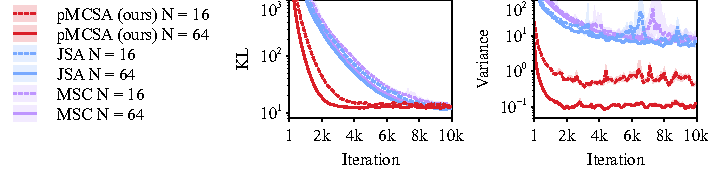
\includegraphics[scale=0.9]{figures/gaussian_02.pdf}
  \vspace{-0.07in}
  \caption{\textbf{
      KL divergence and gradient variance.
      pMCSA not only achieves the least gradient variance, but its variance also scales better with \(N\).
    }
    The target distribution is a 100-D Gaussian with \(\nu = 300\).
    The error bands are the 80\% quantiles while the solid lines are the median of 20 replications.
  }\label{fig:gaussian}
  \vspace{-0.2in}
\end{figure*}

\vspace{-0.05in}
\section{Evaluations}\label{section:eval}

\vspace{-0.05in}
\subsection{Experimental Setup}
\vspace{-0.05in}
\paragraph{Implementation}
For the realistic experiments, we implemented score climbing VI on top of the Turing~\citep{ge2018t} probabilistic programming framework.
For the variational family, we use diagonal Gaussians with the support transformation of~\citet{JMLR:v18:16-107}.
We use the ADAM optimizer by~\citet{kingma_adam_2015} with a learning rate of 0.01 in all of the experiments.
The computational budget is set to \(N=10\) and \(T=2\cdot10^4\) for all experiments unless specified.
We used the mean-field Gaussian variational family for all experiments.

\vspace{-0.1in}
\paragraph{Baselines}
We compare
\begin{enumerate*}[label=\textbf{(\roman*)}]
  \item pMCSA,
  \item JSA,
  \item MSC,
  \item MSC with with Rao-Blackwellization (\textbf{MSC-RB},~\citealt{NEURIPS2020_b2070693}),
  \item adaptive importance sampling (IS) with the self-normalized IS estimator (\textbf{SNIS},~\citealt{robert_monte_2004}), and
  \item evidence lower-bound maximization (\textbf{ELBO},~\citealt{pmlr-v33-ranganath14, JMLR:v18:16-107}) with the path derivative estimator~\citep{NIPS2017_e91068ff}
\end{enumerate*}

\vspace{-0.1in}
\subsection{Simulations}\label{section:simulation}
\vspace{-0.05in}
\paragraph{Target Distribution}
First, we perform experiments on a 100 dimensional correlated multivariate Gaussian where the covariance is sampled from a Wishart distribution with varying degrees of freedom \(\nu\).
This problem is challenging since a IMH/CIS kernel with a diagonal Gaussian proposal will mix very slowly.
Since exact KL divergence between the target and the varitional approximation is available, exact evaluation is possible.

\vspace{-0.1in}
\paragraph{Convergence and Gradient Variance}
The convergence in KL divergence and gradient variance is shown in \cref{fig:gaussian}.
The gradient variance was estimated using \(512\) independent Markov chains using the parameters generated by the main MCSA procedure.
We can see that pMCSA converges the fastest, and benefits the most from increasing \(N\).
This is apparent from the fact that gradient variance dramatically improves by increasing \(N\).
Although other methods also improve slightly by increasing \(N\), the variance reduction is minimal.
This confirms our theoretical analysis in~\cref{section:comparison}.

\vspace{-0.1in}
\paragraph{Robustness Against Optimizers}
We compared the robustness of the MCSA schemes with respect to different SGD optimizers and their hyperparameters in \cref{fig:stepsize}.
Clearly, pMCSA successfully converges for a wider variety of hyperparameters.
Since most methods are the most stable when using ADAM, we use ADAM for all of our remaining experiments.

%% \subsection{Hierarchical Logistic Regression}\label{section:logistic}
%% \vspace{-0.05in}
%% \paragraph{Experimental Setup}
%% We now perform logistic regression with the \texttt{Pima Indians} diabetes (\(\vz \in \mathbb{R}^{11}\),~\citealt{smith_using_1988}), \texttt{German credit} (\(\vz \in \mathbb{R}^{27}\)), and \texttt{heart disease} (\(\vz \in \mathbb{R}^{16}\),~\citealt{detrano_international_1989}) datasets obtained from the UCI repository~\citep{Dua:2019}.
%% 10\% of the data points were randomly selected in each of the 100 repetitions as test data.

% 
\begin{table*}
  \vspace{-0.2in}
  \centering
  \caption{Test Log Predictive Density on Gaussian Process Logistic Classification}\label{table:gp}
  \vspace{-0.05in}
  \setlength{\tabcolsep}{4pt}
  \begin{threeparttable}
  \begin{tabular}{lrrrrrr}
    \toprule
    & \multicolumn{1}{c}{\multirow{2}{*}{ELBO}} & \multicolumn{1}{c}{\multirow{1}{*}{\textbf{pMCSA}}} & \multicolumn{1}{c}{\multirow{2}{*}{JSA}} & \multicolumn{1}{c}{\multirow{2}{*}{CIS}} & \multicolumn{1}{c}{\multirow{2}{*}{CIS-RB}} & \multicolumn{1}{c}{\multirow{2}{*}{SNIS}} \\
    & & \multicolumn{1}{c}{\textbf{(ours)}} & & & & \\
    \midrule
    \textsf{sonar} & {-0.69 {\scriptsize{\(\pm 0.00\)}}} & {\bf-0.68 {\scriptsize{\(\pm 0.00\)}}} & {\bf-0.68 {\scriptsize{\(\pm 0.00\)}}} & {\bf-0.68 {\scriptsize{\(\pm 0.00\)}}} & {\bf-0.68 {\scriptsize{\(\pm 0.00\)}}} & {-0.69 {\scriptsize{\(\pm 0.00\)}}} \\
    \textsf{ionosphere} & {-0.36 {\scriptsize{\(\pm 0.01\)}}} & {\bf-0.35 {\scriptsize{\(\pm 0.01\)}}} & {\bf-0.35 {\scriptsize{\(\pm 0.01\)}}} & {\bf-0.35 {\scriptsize{\(\pm 0.01\)}}} & {\bf-0.35 {\scriptsize{\(\pm 0.01\)}}} & {\bf-0.35 {\scriptsize{\(\pm 0.01\)}}} \\
    \textsf{breast} & {\bf-0.10 {\scriptsize{\(\pm 0.00\)}}} & {-0.11 {\scriptsize{\(\pm 0.01\)}}} & {-0.14 {\scriptsize{\(\pm 0.01\)}}} & {-0.14 {\scriptsize{\(\pm 0.00\)}}} & {-0.14 {\scriptsize{\(\pm 0.01\)}}} & {-0.14 {\scriptsize{\(\pm 0.01\)}}} \\
    \textsf{heart} & {-0.44 {\scriptsize{\(\pm 0.01\)}}} & {\bf-0.43 {\scriptsize{\(\pm 0.01\)}}} & {\bf-0.43 {\scriptsize{\(\pm 0.01\)}}} & {\bf-0.43 {\scriptsize{\(\pm 0.01\)}}} & {\bf-0.43 {\scriptsize{\(\pm 0.01\)}}} & {-0.44 {\scriptsize{\(\pm 0.01\)}}} \\
    \textsf{german} & {\bf-0.48 {\scriptsize{\(\pm 0.01\)}}} & {-0.49 {\scriptsize{\(\pm 0.01\)}}} & {-0.50 {\scriptsize{\(\pm 0.01\)}}} & {-0.50 {\scriptsize{\(\pm 0.01\)}}} & {-0.51 {\scriptsize{\(\pm 0.02\)}}} & {-0.49 {\scriptsize{\(\pm 0.01\)}}} \\
    \textsf{australian} & {\bf-0.21 {\scriptsize{\(\pm 0.01\)}}} & {\bf-0.21 {\scriptsize{\(\pm 0.01\)}}} & {\bf-0.21 {\scriptsize{\(\pm 0.01\)}}} & {\bf-0.21 {\scriptsize{\(\pm 0.01\)}}} & {-0.22 {\scriptsize{\(\pm 0.01\)}}} & {\bf-0.21 {\scriptsize{\(\pm 0.01\)}}} \\\bottomrule
  \end{tabular}
  \begin{tablenotes}
    \item[]{\footnotesize \(\pm\) denotes the 95\% bootstrap confidence intervals obtained from 20 repetitions.}
  \end{tablenotes}
  \end{threeparttable}
  \vspace{-0.15in}
\end{table*}

%%% Local Variables:
%%% TeX-master: "master"
%%% End:



\begin{table*}
  \vspace{-0.1in}
  \centering
  \caption{Test Log Predictive Density on Bayesian Neural Network Regression}\label{table:bnn}
  \vspace{-0.05in}
  \setlength{\tabcolsep}{2pt}
  \begin{threeparttable}
  \begin{tabular}{lrrrcccccc}
    \toprule
    & \multicolumn{1}{c}{\multirow{2}{*}{\(D_{\mathcal{\vlambda}}\)}} & \multicolumn{1}{c}{\multirow{2}{*}{\(D_{\mathcal{\vx}}\)}} &  \multicolumn{1}{c}{\multirow{2}{*}{\(N_{\text{train}}\)}} & \multicolumn{2}{c}{\multirow{1}{*}{ELBO}} & \multicolumn{4}{c}{MCSA Variants} \\\cmidrule(lr){5-6}\cmidrule(lr){7-10}
  & & & & {\footnotesize\(N=1\)} & {\footnotesize\(N=10\)} & \multicolumn{1}{c}{\multirow{1}{*}{\footnotesize{\textbf{pMCSA{\scriptsize\,(ours)}}}}} & \multicolumn{1}{c}{\multirow{1}{*}{\footnotesize{JSA}}} & \multicolumn{1}{c}{\multirow{1}{*}{\footnotesize{CIS}}} & \multicolumn{1}{c}{\multirow{1}{*}{\footnotesize{CIS-RB}}}\\
    \midrule
    \textsf{yacht} & 403 & 6 & 277 & {\bf-2.45 {\scriptsize{\(\pm 0.01\)}}} & {\bf-2.44 {\scriptsize{\(\pm 0.01\)}}} & {\bf-2.49 {\scriptsize{\(\pm 0.01\)}}} & {-3.00 {\scriptsize{\(\pm 0.05\)}}} & {-2.98 {\scriptsize{\(\pm 0.04\)}}} & {-2.98 {\scriptsize{\(\pm 0.04\)}}}\\
    \textsf{concrete} & 503 & 8 & 927 & {-3.25 {\scriptsize{\(\pm 0.01\)}}} & {\bf-3.24 {\scriptsize{\(\pm 0.01\)}}} & {\bf-3.20 {\scriptsize{\(\pm 0.01\)}}} & {-3.33 {\scriptsize{\(\pm 0.02\)}}} & {-3.32 {\scriptsize{\(\pm 0.02\)}}} & {-3.33 {\scriptsize{\(\pm 0.02\)}}}\\
    \textsf{airfoil} & 353 & 6 & 1352 & {-2.53 {\scriptsize{\(\pm 0.02\)}}} & {-2.56 {\scriptsize{\(\pm 0.02\)}}} & {\bf-2.27 {\scriptsize{\(\pm 0.02\)}}} & {-2.51 {\scriptsize{\(\pm 0.02\)}}} & {-2.53 {\scriptsize{\(\pm 0.01\)}}} & {-2.51 {\scriptsize{\(\pm 0.01\)}}}\\
    \textsf{energy} & 503 & 9 & 691 & {-2.42 {\scriptsize{\(\pm 0.02\)}}} & {-2.40 {\scriptsize{\(\pm 0.02\)}}} & {\bf-1.92 {\scriptsize{\(\pm 0.03\)}}} & {-2.38 {\scriptsize{\(\pm 0.02\)}}} & {-2.37 {\scriptsize{\(\pm 0.02\)}}} & {-2.36 {\scriptsize{\(\pm 0.02\)}}}\\
    \textsf{boston} & 753 & 14 & 455 & {\bf-2.72 {\scriptsize{\(\pm 0.03\)}}} & {\bf-2.70 {\scriptsize{\(\pm 0.03\)}}} & {\bf-2.69 {\scriptsize{\(\pm 0.02\)}}} & {-2.82 {\scriptsize{\(\pm 0.02\)}}} & {-2.80 {\scriptsize{\(\pm 0.03\)}}} & {-2.78 {\scriptsize{\(\pm 0.02\)}}}\\
    \textsf{sml} & 1203 & 23 & 3723 & {-1.32 {\scriptsize{\(\pm 0.01\)}}} & {\bf-1.25 {\scriptsize{\(\pm 0.02\)}}} & {\bf-1.22 {\scriptsize{\(\pm 0.01\)}}} & {-1.72 {\scriptsize{\(\pm 0.01\)}}} & {-1.97 {\scriptsize{\(\pm 0.02\)}}} & {-1.95 {\scriptsize{\(\pm 0.02\)}}} \\
    \textsf{gas} & 6503 & 129 & 2308 & {\bf-0.06 {\scriptsize{\(\pm 0.01\)}}} & {\bf 0.13 {\scriptsize{\(\pm 0.03\)}}} & {-0.09 {\scriptsize{\(\pm 0.02\)}}} & {-0.47 {\scriptsize{\(\pm 0.03\)}}} & {-0.47 {\scriptsize{\(\pm 0.04\)}}} & {-0.50 {\scriptsize{\(\pm 0.03\)}}}\\
    \bottomrule
 \end{tabular}
  \begin{tablenotes}
    \item[1] {\footnotesize \(D_{\vlambda}\): Dimentionality of \(\vlambda\), \(D_{\vx}\): Number of features, \(N_{\text{train}}\): Number of training data points.}
    \item[2] {\footnotesize \(\pm\) denotes the 95\% bootstrap confidence intervals obtained from 80 repetitions.}
    \item[3] {\footnotesize Bolded numbers don't have enough evidence to be distinguished from the best performing method under a .05 significance threshold (Friedman test with Nemenyi post-hoc test,~\citealt{JMLR:v7:demsar06a})}.
  \end{tablenotes}
  \end{threeparttable}
  \vspace{-0.1in}
\end{table*}

%%% Local Variables:
%%% TeX-master: "master"
%%% End:



%\begin{wraptable}{r}{0.4\textwidth}
\begin{table*}[t]
  \centering
  \vspace{-2ex}
  \caption{Test Log Predictive Density on \textbf{Robust Gaussian Process Regression}}\label{table:gp}
  \vspace{-1ex}
  %\vspace{-0.05in}
  \setlength{\tabcolsep}{4pt}
  \begin{threeparttable}
  \begin{tabular}{lrrrccccc}
    \toprule
    & \multicolumn{1}{c}{\multirow{2}{*}{\footnotesize\(D_{\vlambda}\)}} & \multicolumn{1}{c}{\multirow{2}{*}{\(D_{\vx}\)}} &  \multicolumn{1}{c}{\multirow{2}{*}{\(N_{\text{train}}\)}} & \multicolumn{1}{c}{\multirow{1}{*}{ELBO}} & \multicolumn{4}{c}{MCSA Variants} \\\cmidrule(lr){5-5}\cmidrule(lr){6-9}
   & & & & \(N=1\) & \multicolumn{1}{c}{\multirow{1}{*}{\footnotesize\textbf{pMCSA{\scriptsize\,(ours)}}}} & \multicolumn{1}{c}{\multirow{1}{*}{\footnotesize{JSA}}} & \multicolumn{1}{c}{\multirow{1}{*}{\footnotesize{MSC}}} & \multicolumn{1}{c}{\multirow{1}{*}{\footnotesize{MSC-RB}}}\\
    \midrule
    \textsf{yacht} & 287 & 6 & 277 & {-3.63 {\scriptsize{\(\pm 0.02\)}}} & {\bf-3.31 {\scriptsize{\(\pm 0.04\)}}} & {\bf-3.29 {\scriptsize{\(\pm 0.05\)}}} & {\bf-3.25 {\scriptsize{\(\pm 0.04\)}}} & {\bf-3.27 {\scriptsize{\(\pm 0.05\)}}} \\
    \textsf{airfoil} & 353 & 6 & 1352 & {-3.14 {\scriptsize{\(\pm 0.01\)}}} & {\bf-2.63 {\scriptsize{\(\pm 0.01\)}}} & {-2.83 {\scriptsize{\(\pm 0.04\)}}} & {-2.77 {\scriptsize{\(\pm 0.02\)}}} & {\bf-2.73 {\scriptsize{\(\pm 0.02\)}}}\\
    \textsf{boston} & 472 & 13 & 455 & {\bf-2.98 {\scriptsize{\(\pm 0.01\)}}} & {\bf-2.96 {\scriptsize{\(\pm 0.02\)}}} & {\bf-3.00 {\scriptsize{\(\pm 0.03\)}}} & {\bf-3.00 {\scriptsize{\(\pm 0.03\)}}} & {\bf-2.96 {\scriptsize{\(\pm 0.03\)}}} \\
    \textsf{energy} & 703 & 8 & 691 & {-2.75 {\scriptsize{\(\pm 0.01\)}}} & {\bf-2.58 {\scriptsize{\(\pm 0.03\)}}} & {-2.78 {\scriptsize{\(\pm 0.04\)}}} & {-2.70 {\scriptsize{\(\pm 0.04\)}}} & {-2.72 {\scriptsize{\(\pm 0.05\)}}} \\
    \textsf{concrete} & 939 & 8 & 927 & {-3.68 {\scriptsize{\(\pm 0.01\)}}} & {\bf-3.49 {\scriptsize{\(\pm 0.01\)}}} & {-3.69 {\scriptsize{\(\pm 0.02\)}}} & {\bf-3.59 {\scriptsize{\(\pm 0.04\)}}} & {\bf-3.57 {\scriptsize{\(\pm 0.02\)}}} \\
    \textsf{wine} & 1454 & 11 & 1439 & {-1.02 {\scriptsize{\(\pm 0.01\)}}} & {\bf-0.94 {\scriptsize{\(\pm 0.02\)}}} & {-1.04 {\scriptsize{\(\pm 0.01\)}}} & {-1.00 {\scriptsize{\(\pm 0.02\)}}} & {-0.99 {\scriptsize{\(\pm 0.02\)}}} \\
    \textsf{gas} & 2440 & 128 & 2308 & {\bf{0.18} {\scriptsize{\(\pm 0.02\)}}} & {\bf-0.86 {\scriptsize{\(\pm 0.02\)}}} & {-1.10 {\scriptsize{\(\pm 0.03\)}}} & {-1.10 {\scriptsize{\(\pm 0.04\)}}} & {-1.06 {\scriptsize{\(\pm 0.02\)}}} 
    \\\bottomrule
  \end{tabular}
  \begin{tablenotes}
    \item[1] {\footnotesize \(D_{\vlambda}\): Dimentionality of \(\vlambda\), \(D_{\vx}\): Number of features, \(N_{\text{train}}\): Number of training data points.}
    \item[2] {\footnotesize \(\pm\) denotes the 95\% bootstrap confidence intervals obtained from 20 replications.}
    \item[3] {\footnotesize Bolded numbers don't have enough evidence to be distinguished from the best performing method under a .05 significance threshold (Friedman test with Nemenyi post-hoc test,~\citealt{JMLR:v7:demsar06a})}.
  \end{tablenotes}
  \end{threeparttable}
  \vspace{-2ex}
\end{table*}
%\end{wraptable}

%%% Local Variables:
%%% TeX-master: "master"
%%% End:


%% %

%% %
%% \begin{wrapfigure}{r}{0.6\textwidth}
%%   \vspace{-0.3in}
%% %\begin{figure}[h]
%%   %\vspace{-0.1in}
%%   %\centering
%%   \subfloat[Test Accuracy]{
%%     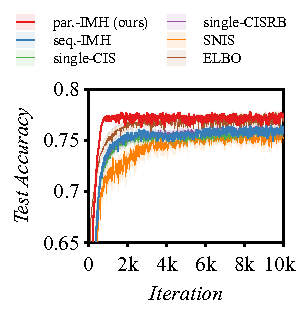
\includegraphics[scale=0.8]{figures/german_02.pdf}\label{fig:german_acc}
%%     \vspace{-0.1in}
%%   } 
%%   %% \subfloat[\texttt{heart}]{
%%   %%   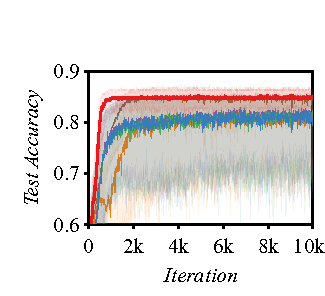
\includegraphics[scale=0.75]{figures/heart_02.pdf}
%%   %% }
%%   %% \subfloat[\texttt{german}]{
%%   %%   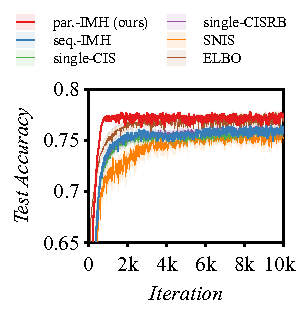
\includegraphics[scale=0.75]{figures/german_02.pdf}
%%   %% }
%%   \subfloat[Test LPD]{
%%     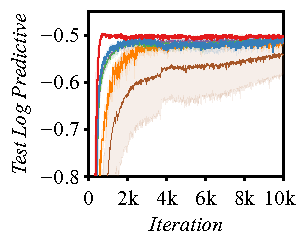
\includegraphics[scale=0.8]{figures/german_03.pdf}\label{fig:german_lpd}
%%     \vspace{-0.05in}
%%   }
%%     \vspace{-0.05in}
%%   \caption{Test accuracy and log predictive density on the \texttt{german} dataset.
%%     The solid lines and colored regions are the mean and 80\% bootstrap confidence interval computed from 100 repetitions.
%%   }\label{fig:logistic}
%%   \vspace{-0.1in}
%% %\end{figure}
%% \end{wrapfigure}
%% %
%% \vspace{-0.05in}
%% \paragraph{Results}
%% The test accuracy and test log predictive density (Test LPD) results are shown in~\cref{table:logistic}.
%% Our proposed parallel state estimator (par.-IMH) achieves the best accuracy and predictive density results.
%% Despite having access to high-quality HMC samples, single-HMC shows poor performance.
%% This supports our analysis that par.-IMH with \(N \geq 2\) superior variance reduction to the single state estimator.
%% Also, seq.-IMH showed poor performance overall due to the correlated samples.
%% Among the two CIS kernel-based methods, single-CISRB performs only marginally better than single-CIS.

%%   \vspace{-0.1in}
%% \paragraph{Inclusive KL v.s. Exclusive KL}
%% While both ELBO and par.-IMH showed similar numerical performance, they chose different optimization paths in the parameter space.
%% This is shown in~\cref{fig:logistic}.
%% While the test accuracy suggests that ELBO converges quickly around \(t=2000\) (\cref{fig:german_acc}), in terms of uncertainty estimate, it takes much longer to converge (\cref{fig:german_lpd}).
%% This shows that inclusive KL minimization chooses a path that has better density coverage as expected.

  \vspace{-0.05in}
\subsection{Gaussian Process Classification}\label{section:bgp}
  \vspace{-0.05in}
\paragraph{Experimental Setup}
For a more challenging problem, we perform classification with latent Gaussian processes~\citep{NIPS2014_8c6744c9}.
The simplified probabilistic model is shown in~\cref{section:gp_logistic} and uses the Mat\'ern 5/2 covariance kernel with automatic relevance determination~\citep{neal_bayesian_1996}.
For the datasets, we use the \texttt{sonar} (\(\vz \in \mathbb{R}^{249}\),~\citealt{gorman_analysis_1988}), \texttt{ionosphere} (\(\vz \in \mathbb{R}^{351}\),~\citealt{Sigillito1989ClassificationOR}), and \texttt{breast} (\(\vz \in \mathbb{R}^{544}\),~\citealt{wolberg_multisurface_1990}) datasets.
For \texttt{breast}, we preprocessed the input features with z-standardization.
10\% of the data points were randomly selected in each of the 100 repetitions as test data.
For this experiment, the iteration complexity of ELBO is almost two orders of magnitude larger than all inclusive KL minimization methods.

%
% \begin{wrapfigure}{r}{0.45\textwidth}
%   \vspace{-0.4in}
%   \centering
%      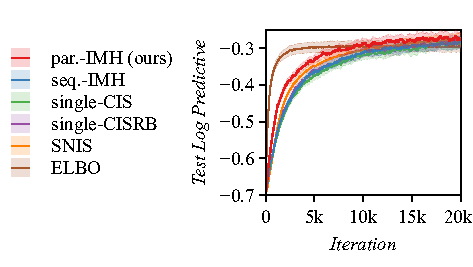
\includegraphics[scale=0.9]{figures/ionosphere_01.pdf}
%   %% \subfloat[\texttt{german}]{
%   %%   \includegraphics[scale=0.75]{figures/breast_01.pdf}
%   %% } \\
%      \vspace{-0.1in}
%   \caption{Test log predictive density on the \texttt{ionosphere} dataset.
%     The solid lines and colored regions are the medians and 80\% percentiles computed from 100 repetitions.
%   }\label{fig:gp}
%   \vspace{-0.2in}
% \end{wrapfigure}
%
\vspace{-0.05in}
\paragraph{Result}
The results are shown in~\cref{table:gp}.
Again, among inclusive KL minimization, our method achieved the best results.
Compared to ELBO, its accuracy was lower on \texttt{breast}, but the uncertainty estimates were much better.
This is better-shown in~\cref{fig:gp}, where ELBO quickly converges to a point with poor uncertainty calibration.
%Meanwhile, on \texttt{breast}, ELBO gives better uncertainty estimates than inclusive KL minimization methods.
%This happens when the modal estimate (preferred by the exclusive KL) gives good accuracy and uncertainty estimates.

%%   \vspace{-0.05in}
%% \subsection{Marginal Likelihood Estimation}\label{section:mll}
%%   \vspace{-0.05in}
%% \paragraph{Experimental Setup}
%% Lastly, we now estimate the marginal log-likelihood of a hierarchical regression model with partial pooling (\texttt{radon}, \(\vz \in \mathbb{R}^{175}\),~\citealt{gelman_data_2007}) for modeling radon levels in U.S homes.
%% \texttt{radon} contains multiple posterior degeneracies from the hierarchy.
%% We estimated the reference marginal likelihood using \textit{thermodynamic integration} (TI,~\citealt{gelman_simulating_1998, neal_annealed_2001, lartillot_computing_2006}) with HMC implemented by Stan~\citep{carpenter_stan_2017, betancourt_conceptual_2017}.
%% %
%% \begin{wrapfigure}{r}{0.45\textwidth}
%%   \vspace{-0.25in}
%%   \centering
%%   \begin{minipage}[b]{0.25\linewidth}
%%     \centering
%%     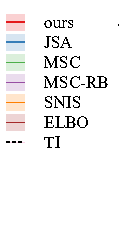
\includegraphics[scale=0.8]{figures/radon_03.pdf}
%%   \end{minipage}
%%   \begin{minipage}[b]{0.7\linewidth}
%%     \centering
%%     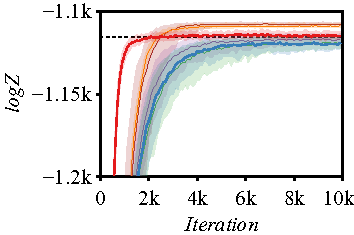
\includegraphics[scale=0.8]{figures/radon_02.pdf}
%%     %\subcaption{\texttt{radon}}
%%   \end{minipage}
%%     \vspace{-0.1in}
%%   %% \begin{minipage}[b]{0.35\linewidth}
%%   %%   \centering
%%   %%   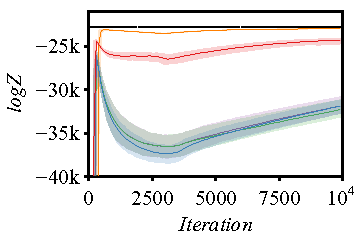
\includegraphics[scale=0.7]{figures/sv_02.pdf}
%%   %%   \subcaption{\texttt{stock}}\label{fig:sv}
%%   %% \end{minipage}
%%   \caption{Marginal log-likelihood estimates on the \texttt{radon} dataset.
%%     The solid lines and colored regions are the medians and 80\% percentiles computed from 100 repetitions.
%%   }\label{fig:marginal_likelihood}
%%   \vspace{-0.2in}
%% \end{wrapfigure}
%
  \vspace{-0.2in}
\paragraph{Results}
The results are shown in~\cref{fig:marginal_likelihood}.
par.-IMH converges quickly and provides the most accurate estimate.
By contrast, other estimators converge much more slowly.
SNIS and ELBO, on the other hand, overestimate \(\log Z\), which can be attributed to the mode-seeking behavior of ELBO and the small sample bias of SNIS.


%%% Local Variables:
%%% TeX-master: "master"
%%% End:
